% !TeX spellcheck = ru_RU
% !TEX root=../main.tex

\begin{lecture}[Общие положения]
	Супрамолекулярная химия является междисциплинарной областью знания, занимая промежуточное место между химией, физикой и биологией.
		
	Тема ,,варения'' новых органических молекул с ковалентными связями уже не так активна, поскольку энергия таких связей будет порядка $-100~\frac{\text{ккал}}{\text{моль}}$.
    Тем не менее, можно создавать новые вещества за счет одинаковых связей (к примеру, водородных, кулоновских, сил Ван-дер-Ваальса), чья энергия порядка
    $ \sim 100 \frac{\text{ккал}}{\text{моль}}$.
    
    Термодинамическая система --- это область пространства, отделенная границей и содержащая частицы.
    При описании состояния системы нужно пользоваться первым началом термодинамики:
    \begin{equation}
    	T dS = dU + p dV,
    	\label{eq:first_statement_therm}
    \end{equation}
    где $U (S, V)$ есть термодинамический потенциал, достигающий минимума в состоянии равновесия.
    
    Нам хотелось уйти от параметра $S$ к другим параметрам в потенциале. Для этого осуществим преобразование Лежандра. В случае точечного преобразования имеем следующий алгоритм:
    \begin{equation}
    	\begin{bmatrix}
			&F( x, y(x), y', y'', \dots ) = 0 & \\
			&\begin{cases}
				t = \alpha (xy) \\
				u = \beta (xy)
			\end{cases}
		% TODO: здесь должна быть нормальная картинка
%		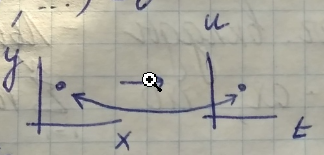
\includegraphics[width=0.15\linewidth]{lecture_01/pic1}
		%--------------------
		\end{bmatrix}
		\label{eq:dot_lejandr}
    \end{equation}
    
    Однако в общем случае преобразование Лежандра не является точечным. Кривая $ y(x) $ может быть задана через производную. В таком случае мы должны изменить наш подход:
    \begin{equation}
    	\begin{bmatrix}
    		&\text{ПЛ не точечное} \\
    		&y(x) \text{ -- кривая (через производную)} \\
    		&\begin{cases}
    			u = y - tx \\
    			t = y_x'
    		\end{cases}
    	\end{bmatrix}
    \end{equation}
    
    Вспомним некоторые термодинамические потенциалы.
    \begin{enumerate}
    	\item $A = U - TS$ --- свободная энергия. Из статистической термодинамики имеем связь $A$ и статистической суммы: $ A = -kT \ln Z $. 
    	\item $ G = H - TS $, $ dG = Vdp - SdT $ (в естественных переменных).
    \end{enumerate}

	Учет химических реакций приводит к определению химического потенциала как добавочного члена вида $ \sum\limits_{i=1}^{N} \mu_i dn_i $, где $ dn_i $ -- количество молей определенного вещества. Если же $ p, T = \text{const} $, то $ dG = \sum\limits_{i=1}{N} \mu_i dn_i $.
	
	\begin{definition}
		Функция однородна степени $n$, если при умножении всех независимых переменных на $k$ мы снова получаем функцию, умноженную на $k^n$. \\
		$ f( kx_1, \dots, kx_N ) = k^n f( x_1, \dots, x_N ) $
	\end{definition}
	
	\begin{theorem}[Эйлера об однородной функции]
		\begin{align}
			f( x_1, \dots, x_N ) &= 0 \rightarrow  k^n f( x_1, \dots, x_N ) \\
			n f( x_1, \dots, x_N ) &= \sum\limits_{i=1}^{N} x_i \dfrac{\partial f}{\partial x_i}
		\end{align}
	\end{theorem}
    
    
    Все термодинамические потенциалы являются однородными функциями 1-ой степени. На основании теоремы Эйлера можно заключить, что
    \begin{equation}
	    \begin{aligned}
    		G = \sum\limits_{i=1}^{N} \mu_i n_i, \tab \mu_i = \left( \dfrac{\partial G}{\partial n_i} \right)_{p, T, n_j (j \neq i)}
	    \end{aligned}
	    \label{eq:G_eiler_combo}
    \end{equation}
    
    Полагается, что выполнено уравнение \textit{Гиббса-Дюгема}: 
    \begin{equation}
		\sum\limits_{i=1}^{N} n_i d\mu_i = 0
		\label{eq:gibbs_dugem}
    \end{equation}
    
    Напоследок отметим, что начальные вклады в развитие этих теорий внесли Льюис, Гиббс и др.
\end{lecture}
